\section{Knowledge Management System}
\label{sec:kms}

We first need to define what is the basic underlying system we build.
How knowledge is compared with data, information, and wisdom.
Then what is knowledge, \ac{KM}, \ac{KMS}, and personal \ac{KMS}.

% --------------------------------------------------
\subsection{Data-Information-Knowledge-Wisdom}

Between data, information, knowledge, wisdom; each of them has their interconnection with each other. Simply put:

\begin{dinglist}{220}
\item Data is the set of facts that already measured
\item Information is the processed data that could be useful (the what, when, where, who)
\item Knowledge is the contextual application of data and information (the how)
\item Wisdom is the evaluated understanding and appreciation of knowledge (the why)
\end{dinglist}

We can even define vision, a future predicted knowledge which is evolved from wisdom.
Figure \ref{fig:kms:dikw-pyramid} illustrates their connection hierarchy as a pyramid structure.

\begin{figure}[htbp]
    \centering
    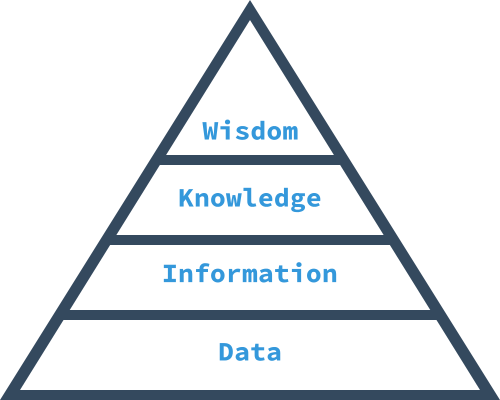
\includegraphics[width=4cm]{\dir/include/dikw-pyramid.png}
    \caption[DIKW Pyramid]{DIKW pyramid illustration about its hierarchy}
    \label{fig:kms:dikw-pyramid}
\end{figure}

% --------------------------------------------------
\subsection{Knowledge}

Generally defined, knowledge is facts, information, and skills acquired by a person through experience or education.
Processed information that bring out insights and undertandings, even processes that can be practiced.
It is the theoretical or practical understanding of a subject, known in a particular field or in total.
Others defined it as an awareness or familiarity gained by experience of a fact or situation.
In general, it is which we are understanding that germinates from combination of data, information, experience, and individual interpretation.~\autocite{BD2015Knowledge}
Knowledge is the
\begin{inparaenum}[\itshape a\upshape)]
\item cognition or recognition (know-what),
\item capacity to act (know-how), and
\item understanding (know-why) that resides or is contained within the mind or in the brain.
\end{inparaenum}
The purpose of knowledge is to better our lives.
In the context of business, the purpose of knowledge is to create or increase value for the enterprise and all its stakeholders.
In short, the ultimate purpose of knowledge is for value creation.~\autocite{Liew2007Understanding}
As well, the roles of knowledge are to
\begin{inparaenum}[\itshape a\upshape)]
\item transform data into information,
\item derive new information from existing ones, and
\item acquire new knowledge pieces
\end{inparaenum}~\autocite{Pomerol2001Relation}

Basically, every information that has a context and are facts can become knowledge.
Some things that could definitely facts are real information about person, organization, product that exists, published media, various places on earth, event that happened or will be held, works in the form of multimedia, etc.
Then up to the circumstances that contained in those knowledge, knowing how they works and more details about them explicitly.

% --------------------------------------------------
\subsection{Knowledge Management}

\ac{KM}\index{knowledge management} could be defined as the process of applying a systematic approach to the capture, structure, management, and dissemination of knowledge throughout an organization in order to work faster, reuse best practices, and reduce costly rework from project to project.~\autocite{Dalkir2005KM}
\ac{KM} itself has already been created before its term exist, since the era of industrialization (circa 1800) and mostly used for corporate necessities.
Hence, \ac{KM} can be performed without the help of a computer, with just manual operation by human.

\begin{figure}[htbp]
    \centering
    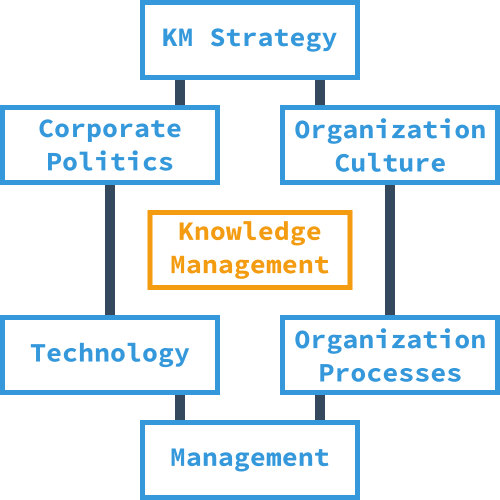
\includegraphics[width=5cm]{\dir/include/km-dimensions}
    \caption{Knowledge Management Dimensions}
    \label{fig:kms:dimensions}
\end{figure}

As knowledge management is essentially about getting the right knowledge to the right person at the right time~\autocite{Frost2010KM}, there are various factors around \ac{KM} that must be noted like in \autoref{fig:kms:dimensions}:

\begin{description}
  \item [KM Strategy]: The objective to take care of knowledge assets
  \item [Organizational Culture]: The influence of people interaction
  \item [Organizational Processes]: The implementation enabler
  \item [Management \& Leadership]: The competent and experienced team
  \item [Technology]: The systems, tools, and technologies that fit the requirements
  \item [Politics]: The long-term support to implement and sustain initiatives
\end{description}

Effective knowledge management changes the way organizations and individuals function.
It changes the way individuals go about their daily tasks, and this correlates to changes in the organization’s values and beliefs.~\autocite{Call2005KM}
Therefore, \ac{KM} is about making knowledge-based work tasks or daily life more effective, if it is a good knowledge management.
Good knowledge management is all about getting the right knowledge, in the right place, at the right time.~\autocite{Brun:2015:ABCKM:6}
Although every things or features that needed may vary for each organizations and invididuals.

% --------------------------------------------------
\subsection{Knowledge Management System}

\ac{KMS}\index{knowledge management system} that also can be referred as a knowledge manager, is a set of methods for the improvement of business or even daily process performance within the scope of knowledge management.
It is most often used in business in applications such as information systems, business administration, computer science, public policy, and general management.
Common company departments for knowledge management systems include human resources, business strategy, and information technology.~\autocite{BD2015KMS}
In short, \ac{KMS}s are tools aimed at supporting knowledge management.~\autocite{Dalkir2005KM}
Nowadays \ac{KMS} can be handled with a great deal of computer system, network, and people together.
Knowledge management systems are one of the key strategies that allow companies to fully tap into their collective knowledge.~\autocite{Panela2011mikrow}

In this context, it is also could be more and beyond that, because \ac{KMS} can:

\begin{easylist}
& Comprises a range of practices used in an organization to identify, create represent distribute and enable adoption to insight and experience
& Be such insights and experience comprise knowledge, either embodied in individual or embedded in organizational processes and practices.
\end{easylist}

So it is the thing of storing and managing these kinds of knowledge in a decent friendly ecosystem that has:

\begin{easylist}
& Personalized information
& State of knowing and understanding
& Object to be stored and manipulated
& Process of applying expertise
& Condition of access to information
& Potential to influence action
\end{easylist}

% --------------------------------------------------
\subsection{Personal {KMS}}

It is simply defined as the simplified and minimized version of \ac{KMS}, kind of based on what commonly called micro \ac{KMS}.
The micro approach allow us to start the system as small as possible but still possible to be enlarged and adapted into any size.
But unlike any other concept and implementation of commonly defined as micro knowledge management system, personal \ac{KMS} procedure takes on the essence of the user scale, which is personal.
In a simple matter, personal \ac{KMS} has a very small scope as in user, system, and architecture size.
Effectively, personal \ac{KMS} is used for daily knowledge management, but also capable of managing tons of knowledge.
Those kind of knowledge are including everyday knowledge such as personal profiles, organization profiles, product details, publications, places, events, multimedia pieces, and miscellaneous things.
So it is somewhat different with regular \ac{KMS} that is mostly used only by organization, that is usually has a large business.
Even though, if for example every person in an organization (potentially small to medium size business), personal \ac{KMS} can also be a collective or regular \ac{KMS}.
Personal \ac{KMS} can also be referred as a personal knowledge manager.

% --------------------------------------------------
\subsection{Knowledge Base}

Explaining a bit about \ac{KB}\index{knowledge base} and how it is different from \ac{KMS} can be likened as comparing encyclopedia and comprehensive library with various type of contents.
\ac{KB} is like encyclopedia, mostly storing just collection of information without concerning much about process and meaning.
But \ac{KMS} is like comprehensive library, more into collection of knowledge that can be used with and processed for specific context, because there are plenteous of them ranging from stories to catalogues to tutorials.
Also, \ac{KB} is closely related to database while \ac{KMS} can even be done without a database but just collections of knowledge in various formats and sources.
\ac{KB} is likewise related to expert system, a system which depends on \ac{KB} for its substantial informations.
In conclusion, \ac{KB} encompasses the technology for storing all kinds of information and knowledge that oftentimes using computer system.
